\documentclass[pdflatex,sn-mathphys-num]{sn-jnl}
\usepackage{graphicx}
\usepackage{booktabs}
\usepackage{multirow}
\usepackage{longtable}
\usepackage{array}
\usepackage{siunitx}
\usepackage{url}
\usepackage{float}

\jyear{2026}

\title[Cross-tribe phenotypic and behavioral structure]{Integrated cross-tribe phenotypic, behavioral, and dermatoglyphic profiling from community survey workbooks}

\author*[1]{\fnm{Ranji} \sur{Kolkar}}\email{ranji.kolkar@example.com}
\author[1]{\fnm{Swea} \sur{Nidhi}}\email{swea.nidhi@example.com}

\affil[1]{\orgname{Independent Research Collaboration}, \orgaddress{\city{Goa}, \country{India}}}

\abstract{\n
Population-scale profiling of underserved tribal communities often remains fragmented across administrative, anthropometric, and biosample spreadsheets, limiting integrated interpretation. We present a reproducible analytical pipeline for two tribe-level datasets (Nirankal and Virnoda) represented across roster, anthropometric, questionnaire, and fingerprint-hair sheets. The framework harmonizes schema inconsistencies, quantifies missingness, and performs multi-layer inference across demographic, body-composition, lifestyle, and dermatoglyphic dimensions. Statistical inference combines Mann-Whitney U testing, chi-square association testing, effect-size estimation (Cohen's \(d\), Cliff's delta, Cramer's \(V\)), and false-discovery-rate control. Pattern discovery layers include principal component analysis and bilateral fingerprint symmetry metrics. Across 188 roster entries, Virnoda showed consistently higher central tendency for BMI and most body-circumference variables, but with predominantly small standardized effect sizes. Behavioral divergence was strongest for tobacco-use responses. Dermatoglyphic signatures revealed shared dominant classes (W, UL, PA) but markedly different repertoire diversity (Shannon entropy 3.205 in Nirankal versus 2.179 in Virnoda). These findings illustrate that tribe-level differences are better represented as multivariate profile shifts rather than single-variable contrasts. We provide a full manuscript-ready artifact suite with figures, statistical tables, and a transparent methodology diagram designed for auditability and reuse.
}

\keywords{tribal health, anthropometry, dermatoglyphics, behavioral epidemiology, multivariate statistics, reproducible analytics}

\begin{document}
\maketitle

\section{Introduction}
Indigenous and tribal populations are frequently analyzed through narrow, single-domain snapshots, while real-world survey operations generate richer but structurally heterogeneous data streams spanning family rosters, anthropometry, questionnaire responses, and biological or forensic descriptors. This disconnect between data collection breadth and analytic integration can obscure meaningful cross-group structure. Robust statistical synthesis in such settings requires careful harmonization, explicit treatment of missingness, and effect-size-centric inference rather than reliance on \(p\)-values alone \cite{rubin1976,little2002,vanbuuren2018,cohen1988,cliff1993}.

Anthropometry remains a central proxy for nutrition and cardiometabolic risk at population scale \cite{who1995,who2000,wells2006}. Questionnaire indicators, especially tobacco and alcohol use, provide complementary behavioral context relevant to chronic disease trajectories. Dermatoglyphic profiles, while historically used in population anthropology and biometric science \cite{galton1892,henry1900,cummins1961,holt1968}, are less frequently analyzed jointly with contemporary community health indicators.

From a methodological perspective, modern quantitative workflows emphasize non-parametric inference when normality assumptions are uncertain \cite{mann1947,wilcoxon1945}, association modeling for categorical structure \cite{agresti2013,cramer1946}, and multiplicity control through false-discovery-rate procedures \cite{benjamini1995}. Pattern-level dimensionality reduction (PCA) complements these tests by identifying latent geometric organization across correlated measurements \cite{pearson1901,hotelling1933,jolliffe2002,kaiser1960}.

In this study, we integrate two tribe workbooks (Nirankal and Virnoda) into a unified analytical framework and present a full manuscript-ready output package. Our goals are fourfold: (i) quantify cross-tribe commonalities and divergences across demographic, anthropometric, behavioral, and dermatoglyphic layers; (ii) report both statistical significance and practical effect sizes; (iii) benchmark data quality and missingness explicitly; and (iv) provide a reproducible, publication-oriented workflow and visualization set.

\section{Contributions}
This work makes the following contributions:
\begin{enumerate}
\item A reproducible, multi-sheet harmonization pipeline converting heterogeneous Excel survey workbooks into analysis-ready panel data.
\item An integrated inferential stack combining Mann-Whitney U, chi-square, Cramer's \(V\), Cohen's \(d\), Cliff's delta, and Benjamini-Hochberg correction.
\item A dermatoglyphic diversity and bilateral-symmetry layer that extends beyond conventional demographic-anthropometric analysis.
\item A publication-ready artifact suite with methodology diagram, seven quantitative figures, and six structured result tables.
\item A Nature-style LaTeX manuscript scaffold suitable for direct extension into journal submission packages.
\end{enumerate}

\section{Methods}
\subsection{Data sources and harmonization}
Two workbooks were analyzed: \textit{Nirankal Tribe List.xlsx} and \textit{Virnoda Tribe List.xlsx}. Sheets were mapped to four principal analytical domains: roster, measurements, questionnaire, and fingerprint-hair. Column-level normalization addressed common operational inconsistencies (for example, trailing spaces in sheet names, mixed-case categorical labels, and numeric coercion of anthropometric fields).

All-cells-empty rows were removed. Roster age values were converted to numeric with non-coercible values treated as missing. Categorical values were uppercased and whitespace-normalized prior to contingency analyses. Fingerprint records were transformed into long format for per-code composition statistics.

\subsection{Methodology workflow diagram}
Figure~\ref{fig:method} summarizes the complete pipeline from ingestion to publication artifacts.

\begin{figure}[H]
\centering
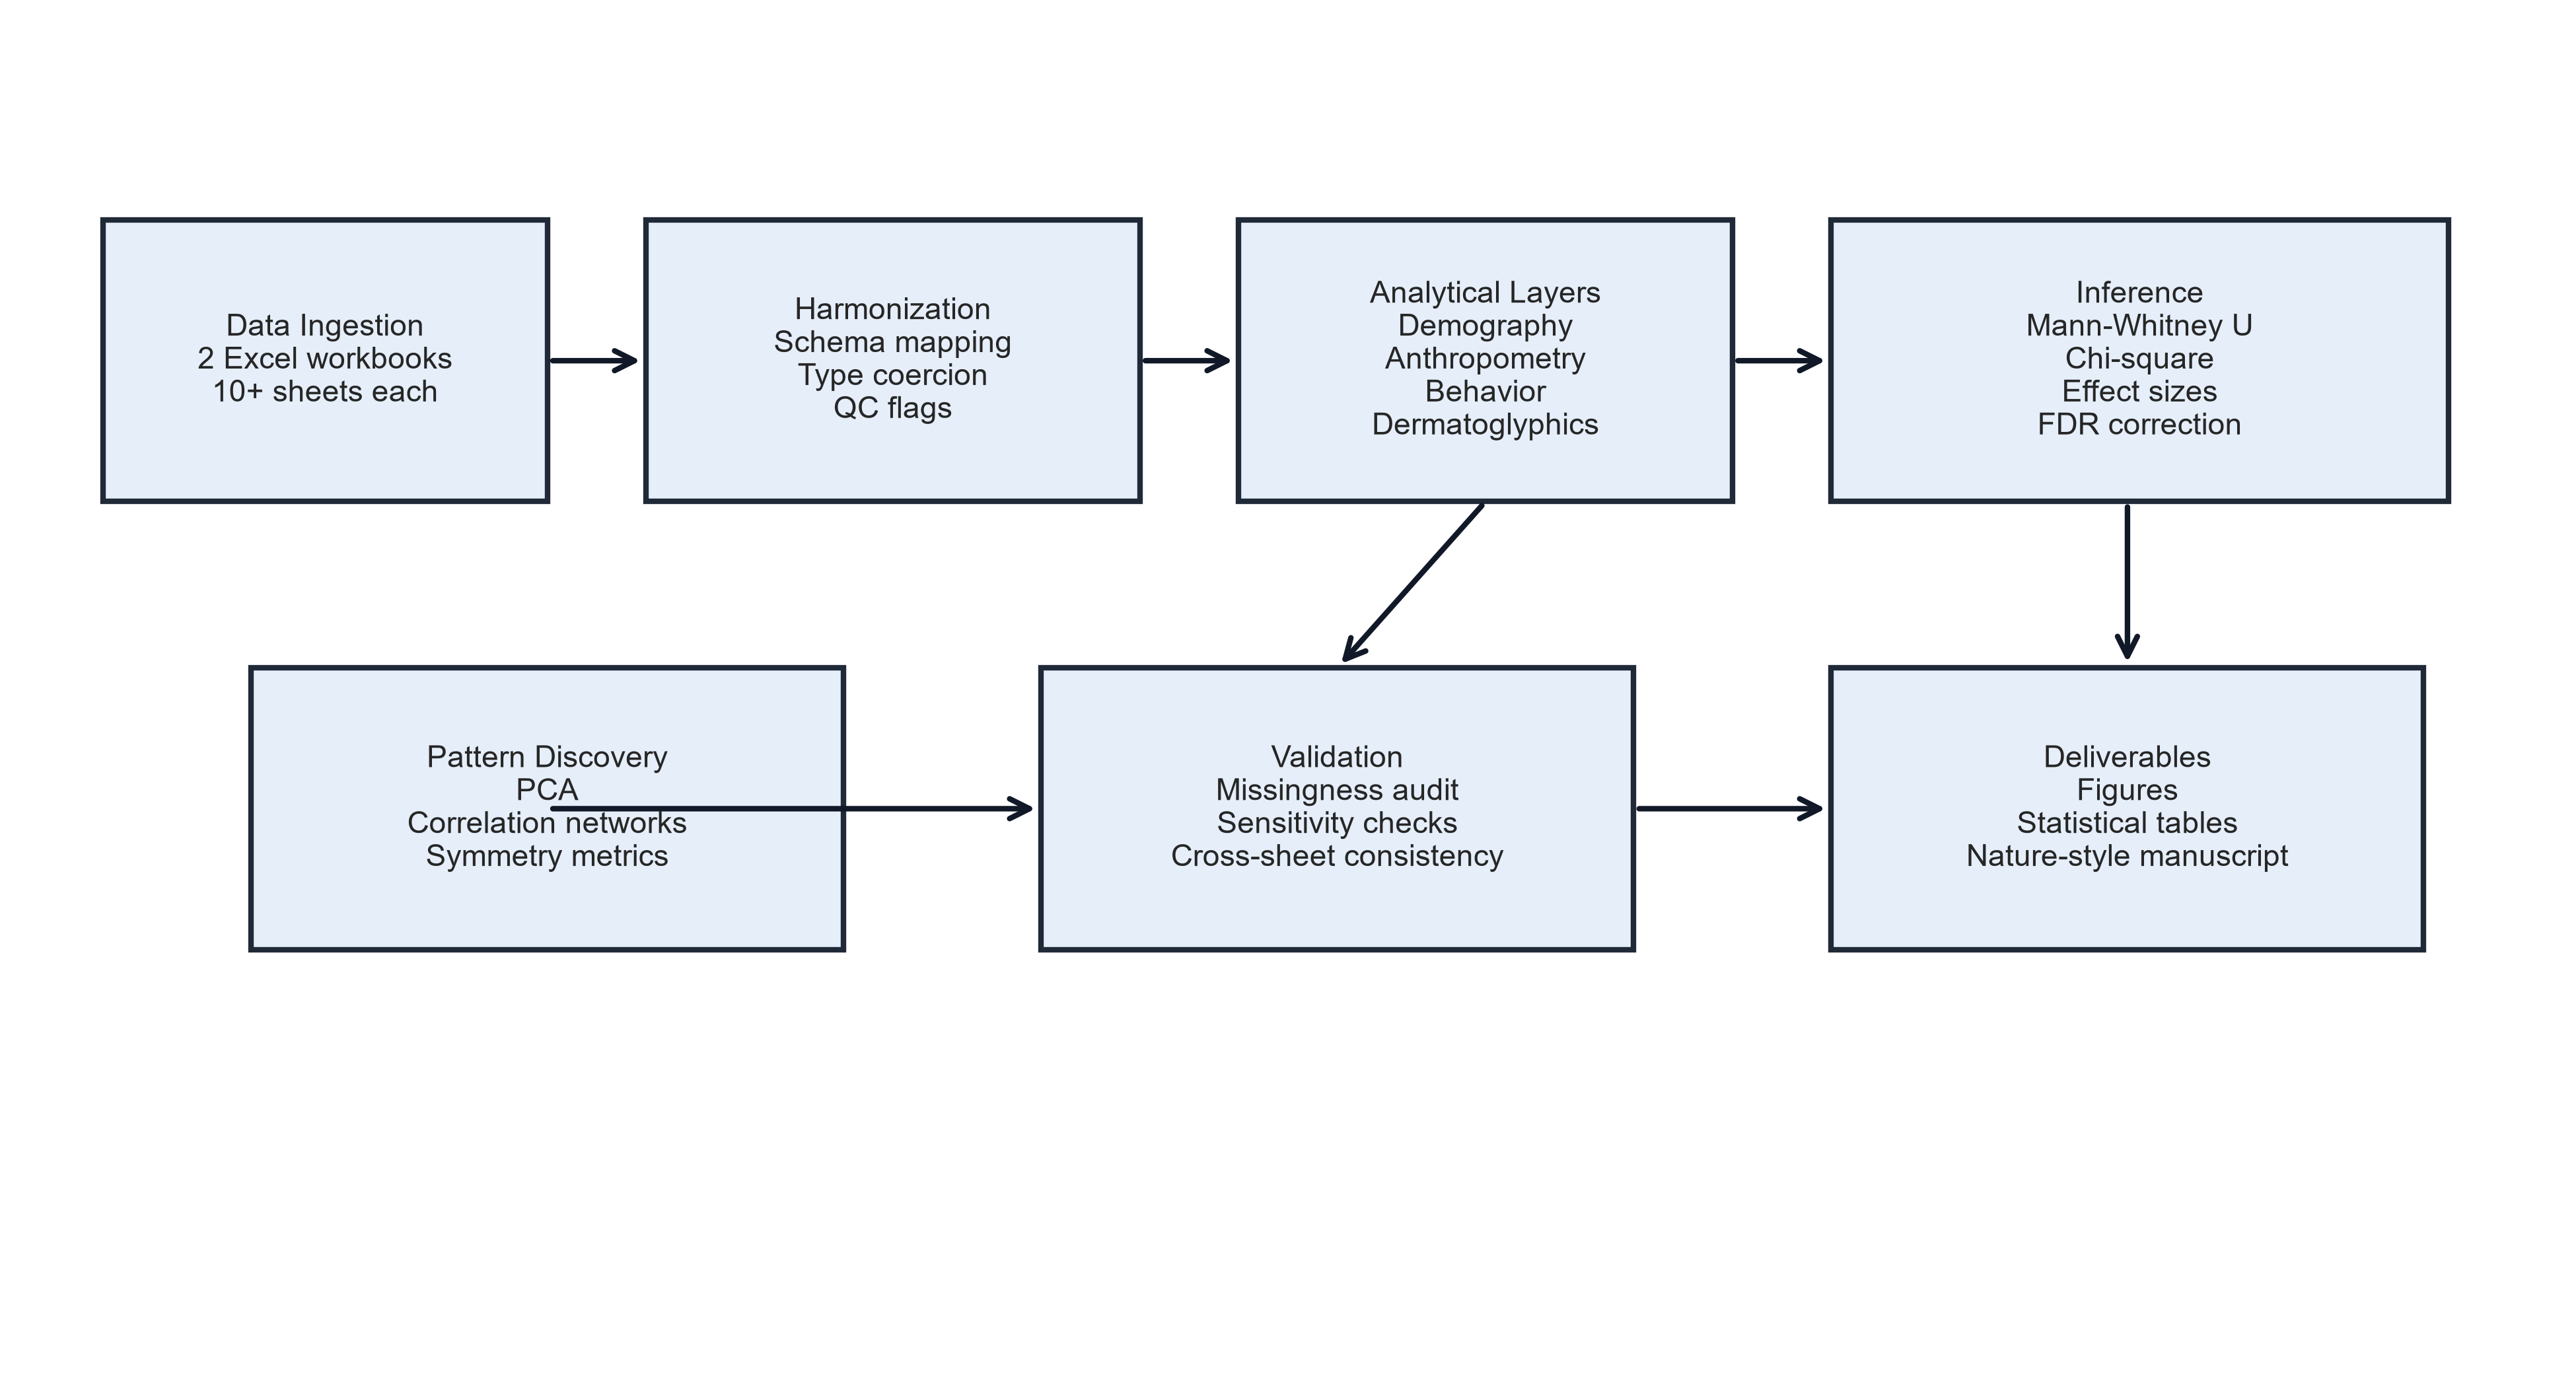
\includegraphics[width=0.98\textwidth]{figures/methodology_pipeline.png}
\caption{End-to-end methodology pipeline. Data ingestion and harmonization are followed by layered analysis (demography, anthropometry, behavior, dermatoglyphics), inferential statistics with multiplicity control, pattern-discovery methods (PCA and symmetry metrics), validation checks, and manuscript-ready outputs.}
\label{fig:method}
\end{figure}

The diagram encodes six operational stages: ingestion, harmonization, analytical layering, inference, validation, and deliverable generation. This structure ensures that inferential claims are linked to upstream preprocessing assumptions and downstream reproducibility outputs.

\subsection{Statistical techniques}
We used a mixed inferential strategy designed for heterogeneous real-world data:
\begin{enumerate}
\item \textbf{Non-parametric two-sample comparison}: Mann-Whitney U for continuous anthropometric variables \cite{mann1947,wilcoxon1945}.
\item \textbf{Categorical association}: Chi-square tests over tribe-by-category contingency tables \cite{agresti2013}.
\item \textbf{Effect-size reporting}: Cohen's \(d\) for standardized mean shift \cite{cohen1988}, Cliff's delta for ordinal/non-parametric effect \cite{cliff1993}, and Cramer's \(V\) for categorical strength \cite{cramer1946}.
\item \textbf{Multiplicity control}: Benjamini-Hochberg FDR correction across each family of tests \cite{benjamini1995}.
\item \textbf{Pattern discovery}: PCA on standardized anthropometric variables \cite{pearson1901,hotelling1933,jolliffe2002,kaiser1960}.
\item \textbf{Information-theoretic diversity}: Shannon entropy of fingerprint code distributions \cite{shannon1948}.
\end{enumerate}

\subsection{Software and reproducibility}
The pipeline was implemented in Python using NumPy \cite{harris2020}, pandas \cite{mckinney2010}, SciPy \cite{virtanen2020}, scikit-learn \cite{pedregosa2011}, Matplotlib \cite{hunter2007}, and seaborn \cite{waskom2021}. Scripts produce all figures and tables under a dedicated asset directory.

\section{Results}
\subsection{Cohort structure and demographic baseline}
Combined roster size was 188 individuals: 120 in Nirankal and 68 in Virnoda. Median age was similar (17 vs 18 years), but interquartile age spread was wider in Nirankal (Table~\ref{tab:cohort}). Age-sex banding (Figure~\ref{fig:agesex}) indicates a stronger early-age female concentration in Nirankal and a more balanced younger structure in Virnoda.

\begin{table}[H]
\centering
\caption{Cohort profile by tribe.}
\label{tab:cohort}
\begin{tabular}{lrrrrr}
\toprule
Tribe & Roster \(n\) & Male & Female & Median age & Age IQR \\
\midrule
Nirankal & 120 & 56 & 64 & 17.0 & 29.0 \\
Virnoda & 68 & 36 & 32 & 18.0 & 20.0 \\
\bottomrule
\end{tabular}
\end{table}

\begin{figure}[H]
\centering
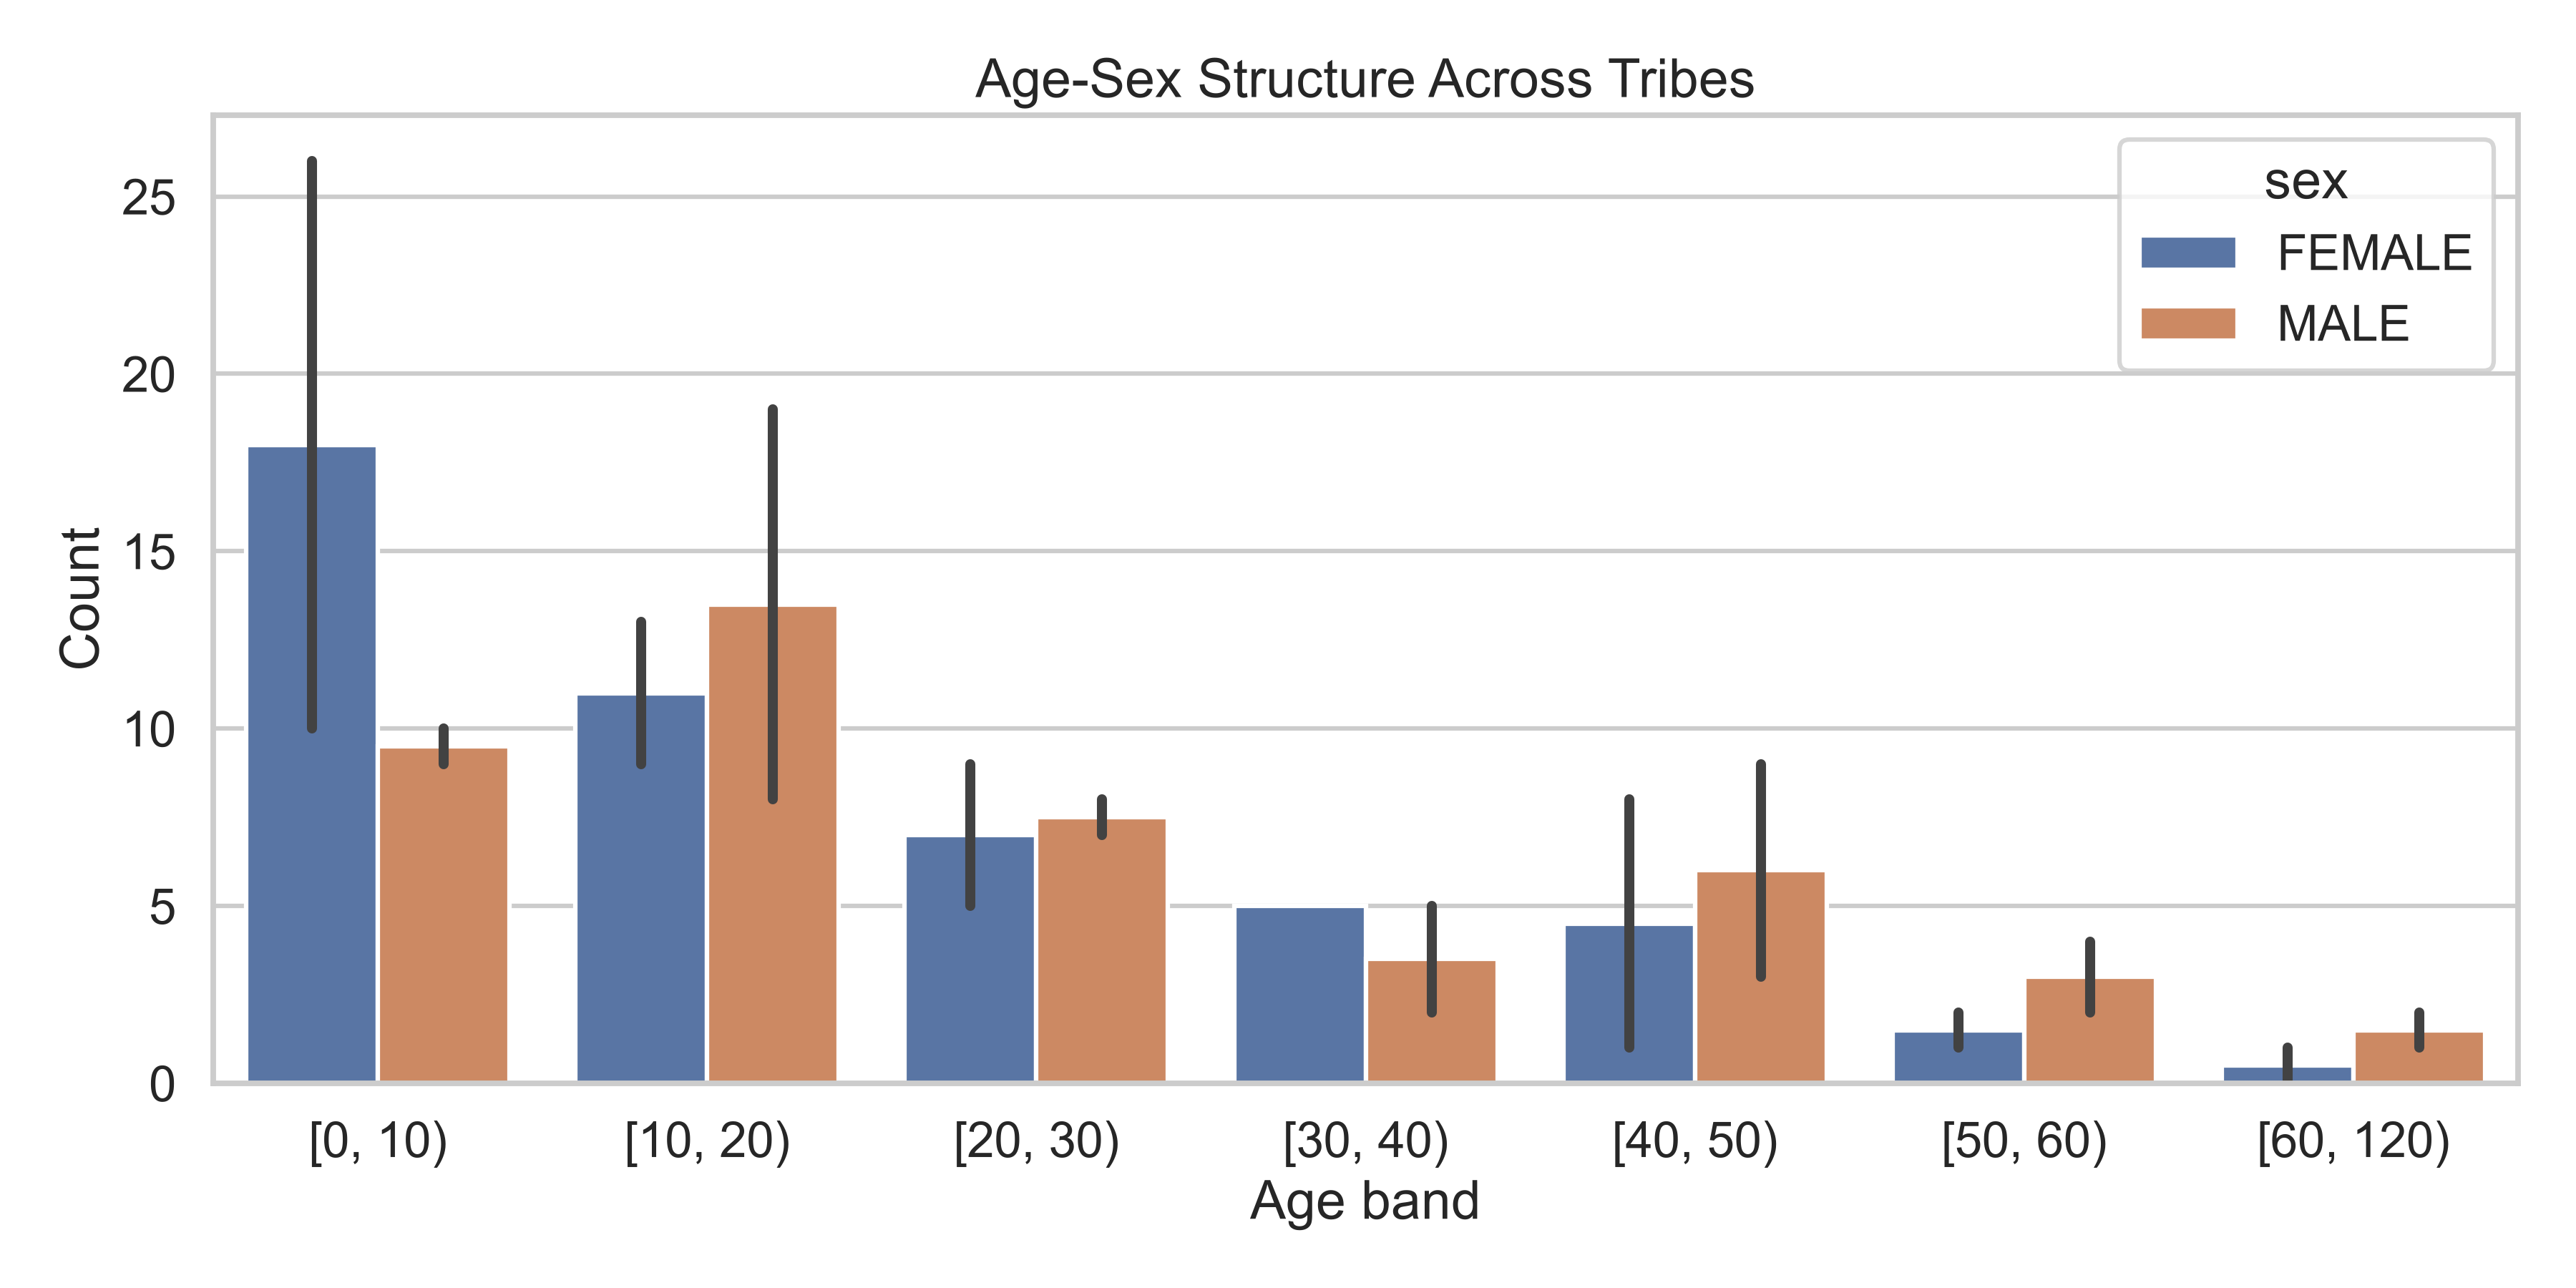
\includegraphics[width=0.9\textwidth]{figures/age_sex_structure.png}
\caption{Age-sex structure across tribes.}
\label{fig:agesex}
\end{figure}

\subsection{Anthropometric contrasts and standardized effects}
Anthropometric medians were generally higher in Virnoda across BMI and circumference variables, but standardized shifts were mostly small (Table~\ref{tab:anthro}). The strongest nominal contrast occurred for biceps thickness (\(p=0.021\), unadjusted), although this did not remain significant after FDR adjustment (\(q=0.234\)). Figure~\ref{fig:effect} and Figure~\ref{fig:bmi} show the effect-size profile and BMI distributions, respectively.

\begin{table}[H]
\centering
\caption{Anthropometric two-sample inference and effect sizes (Virnoda relative to Nirankal).}
\label{tab:anthro}
\scriptsize
\begin{tabular}{lrrrrrr}
\toprule
Variable & Median (Nir) & Median (Vir) & \(p\) & \(q_{BH}\) & Cohen's \(d\) & Cliff's \(\delta\) \\
\midrule
Biceps (mm) & 27.4 & 22.0 & 0.0213 & 0.2342 & -0.364 & 0.255 \\
BMI & 15.95 & 17.60 & 0.0936 & 0.4009 & 0.269 & -0.225 \\
Triceps (mm) & 26.43 & 21.50 & 0.1912 & 0.4009 & -0.233 & 0.145 \\
Height (cm) & 139.45 & 146.51 & 0.2651 & 0.4009 & 0.137 & -0.124 \\
Chest Cir (cm) & 68.38 & 72.00 & 0.2806 & 0.4009 & 0.164 & -0.120 \\
Waist Cir (cm) & 58.30 & 62.00 & 0.2967 & 0.4009 & 0.207 & -0.116 \\
Weight (kg) & 33.29 & 38.10 & 0.3024 & 0.4009 & 0.231 & -0.114 \\
Hip Cir (cm) & 70.39 & 77.20 & 0.3149 & 0.4009 & 0.236 & -0.111 \\
Subscapular (mm) & 11.98 & 10.50 & 0.3280 & 0.4009 & -0.107 & 0.109 \\
Head Cir (cm) & 50.39 & 50.00 & 0.9338 & 0.9592 & 0.017 & 0.010 \\
Abdomen (mm) & 14.50 & 13.90 & 0.9592 & 0.9592 & 0.079 & 0.006 \\
\bottomrule
\end{tabular}
\end{table}

\begin{figure}[H]
\centering
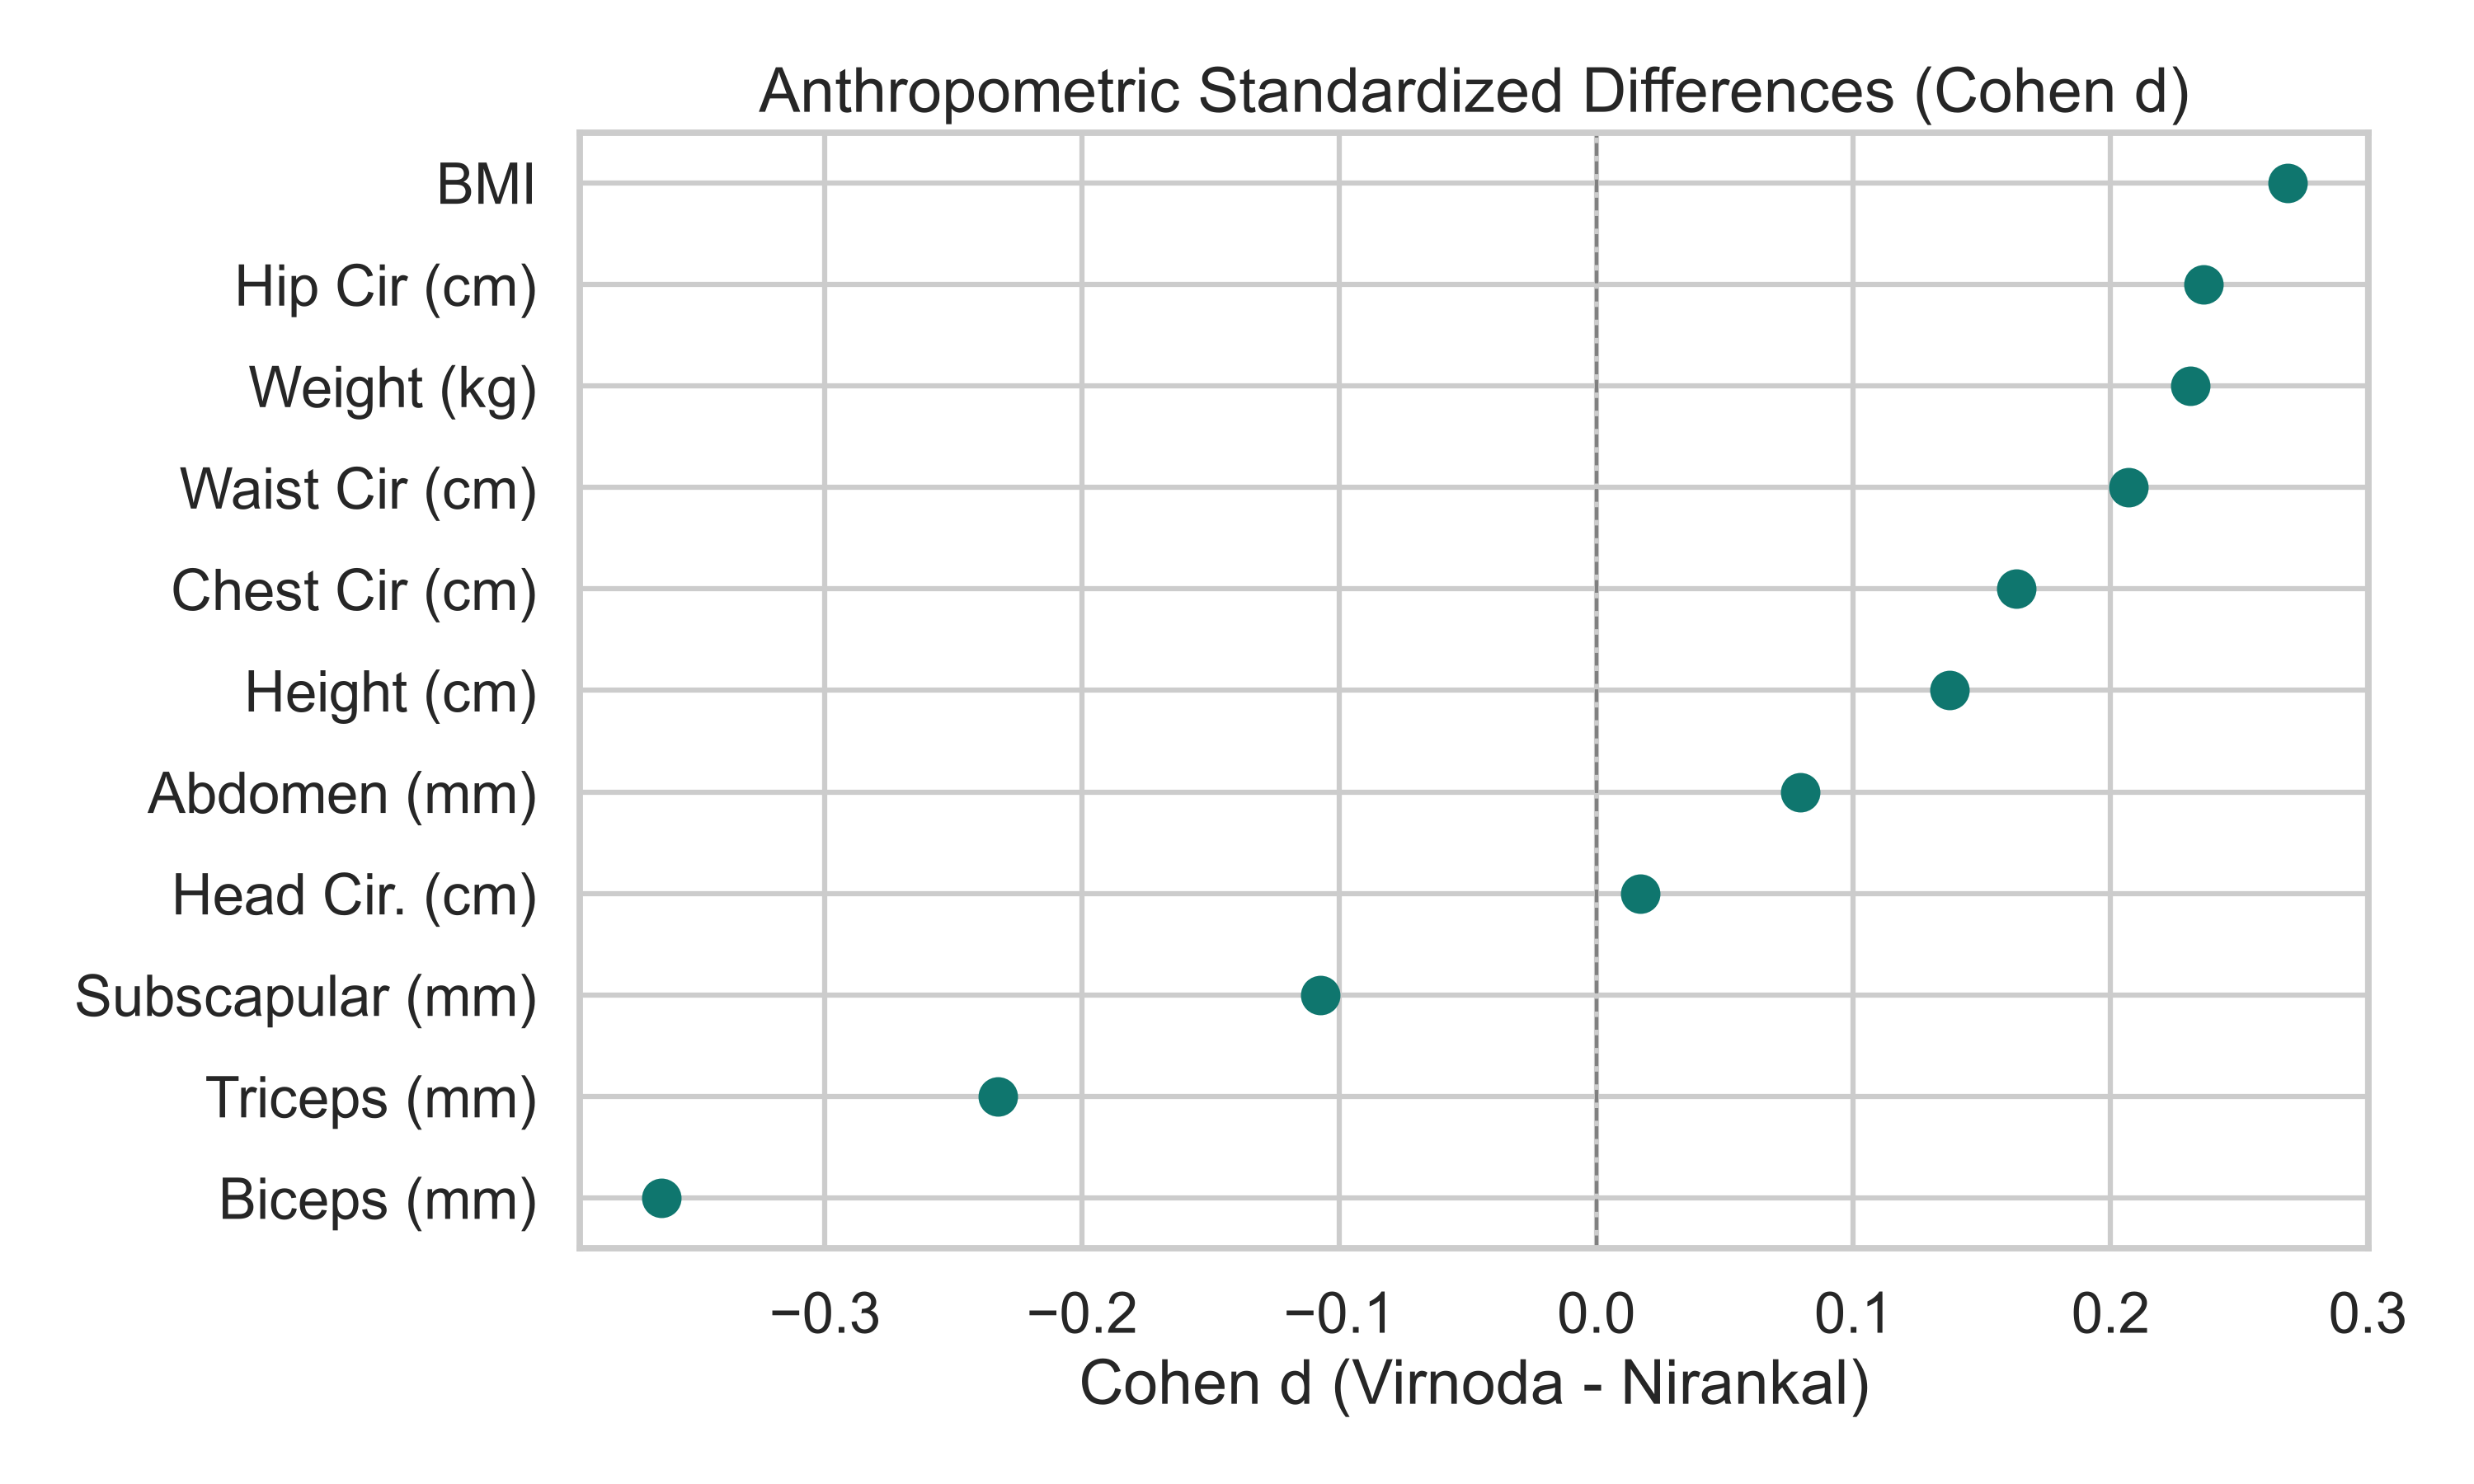
\includegraphics[width=0.88\textwidth]{figures/effect_sizes_cohens_d.png}
\caption{Anthropometric standardized differences (Cohen's \(d\), Virnoda minus Nirankal).}
\label{fig:effect}
\end{figure}

\begin{figure}[H]
\centering
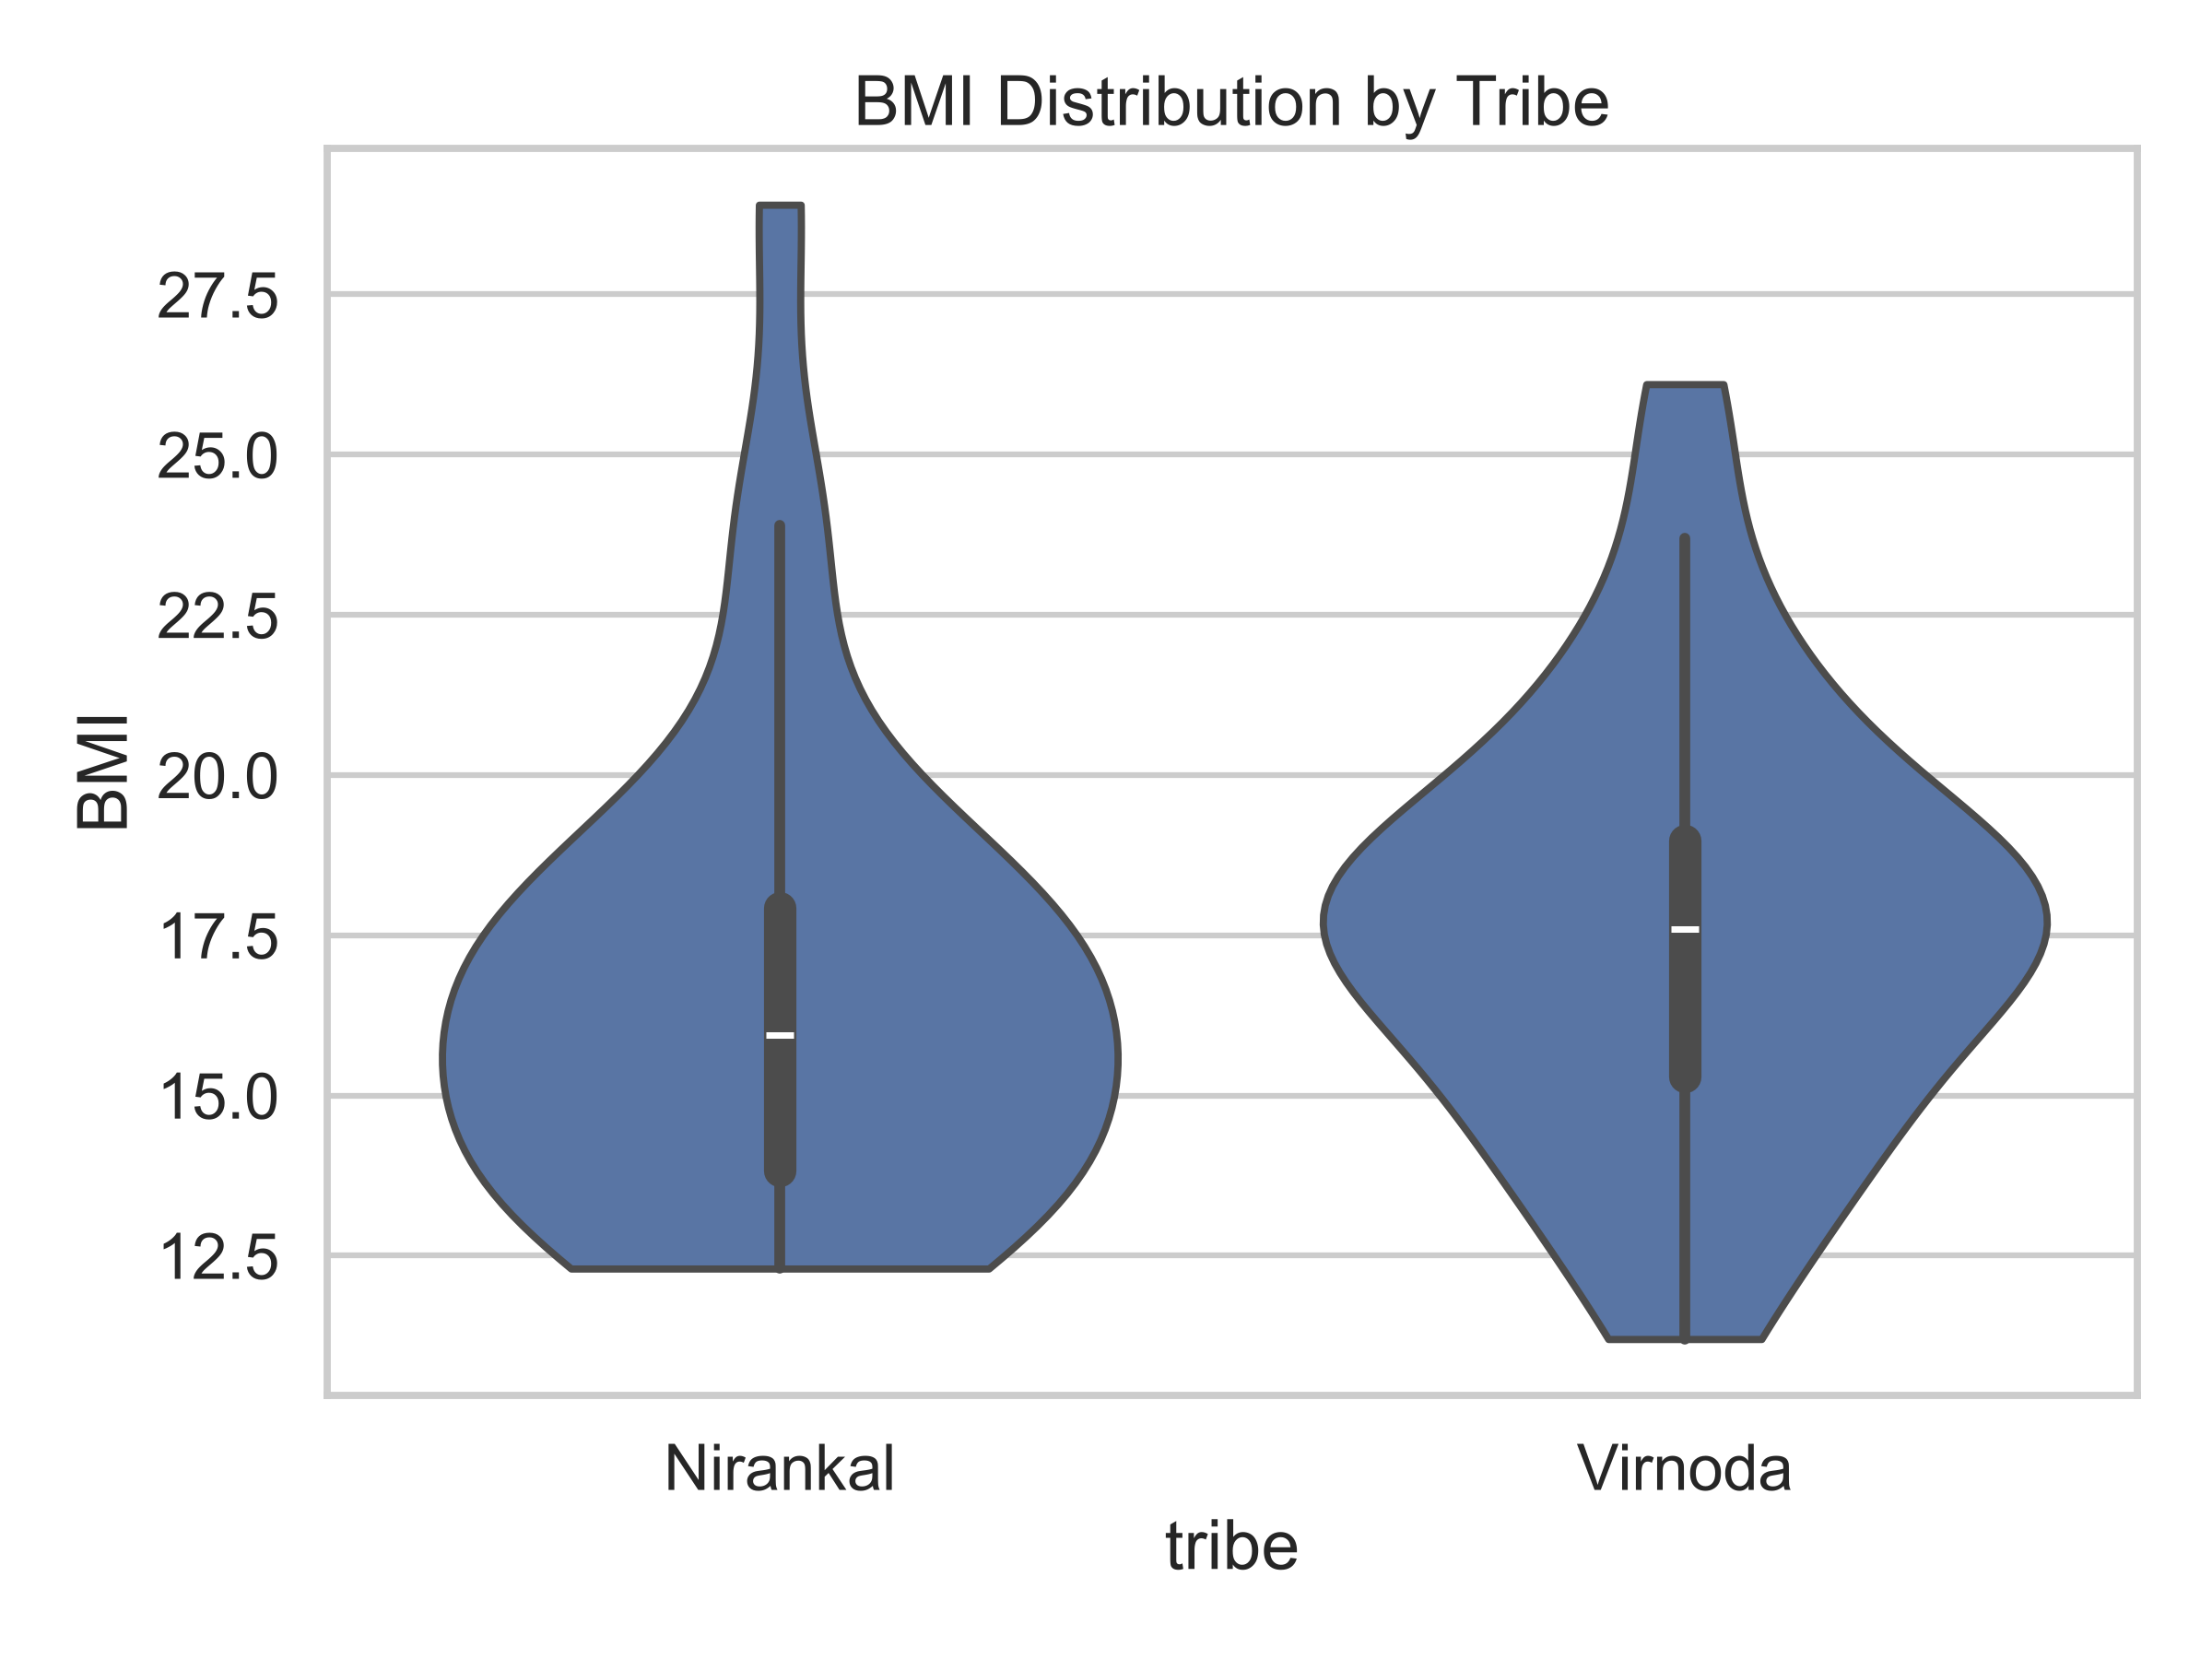
\includegraphics[width=0.70\textwidth]{figures/bmi_violin.png}
\caption{BMI distribution by tribe.}
\label{fig:bmi}
\end{figure}

\subsection{Behavioral and socioeconomic response structure}
Questionnaire structure differed most in work and tobacco categories (Table~\ref{tab:cat}). Main-work responses showed the strongest categorical divergence (\(\chi^2=19.0\), \(q<0.001\), Cramer's \(V=1.0\), though with limited effective \(n\) due to sparsity). Tobacco-use divergence was also strong (\(\chi^2=16.09\), \(q<0.001\), Cramer's \(V=0.463\)). Figure~\ref{fig:behav} summarizes non-\textit{never} exposure rates.

\begin{table}[H]
\centering
\caption{Categorical association tests across tribes.}
\label{tab:cat}
\begin{tabular}{lrrrrr}
\toprule
Field & \(\chi^2\) & dof & \(p\) & \(q_{BH}\) & Cramer's \(V\) \\
\midrule
Main Work & 19.000 & 2 & 0.0000749 & 0.000374 & 1.000 \\
Tobacco Smoke Use & 16.087 & 2 & 0.000321 & 0.000803 & 0.463 \\
Marital Status & 4.909 & 3 & 0.1786 & 0.2322 & 0.238 \\
Alcohol Use Frequency & 3.366 & 2 & 0.1858 & 0.2322 & 0.204 \\
Education & 5.491 & 6 & 0.4825 & 0.4825 & 0.349 \\
\bottomrule
\end{tabular}
\end{table}

\begin{figure}[H]
\centering
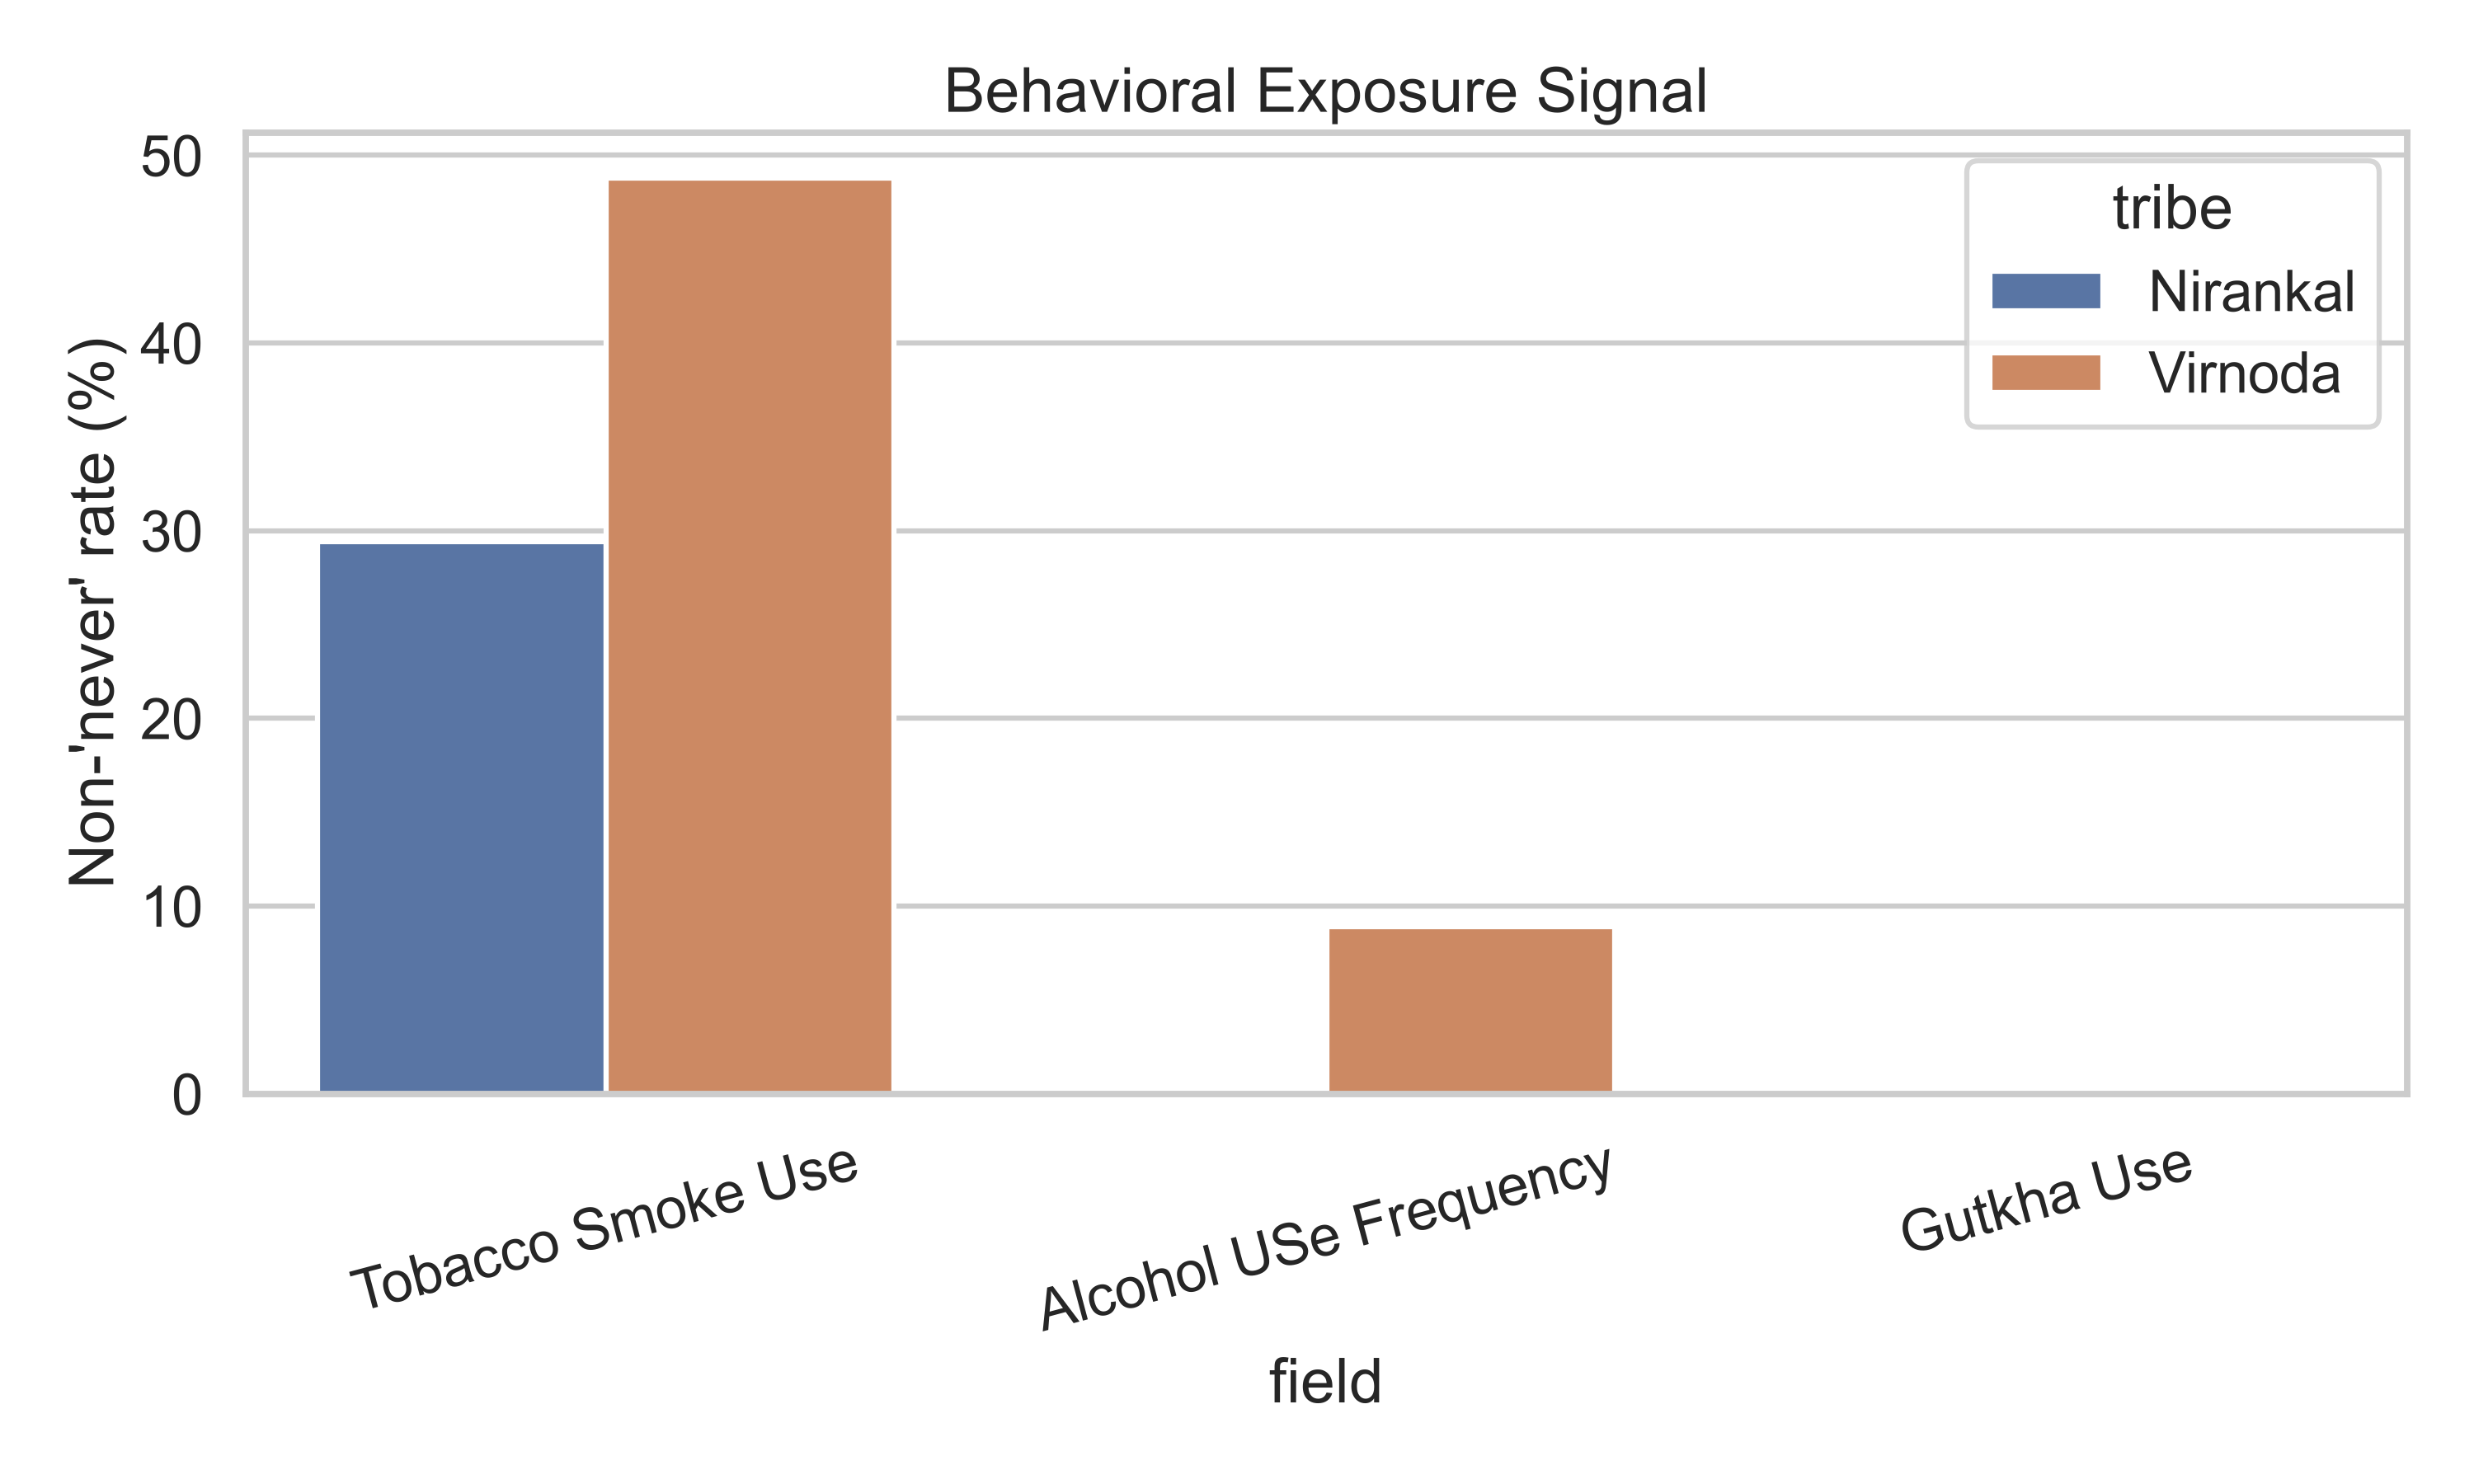
\includegraphics[width=0.88\textwidth]{figures/behavior_non_never_rates.png}
\caption{Behavioral exposure signal represented as non-\textit{never} response rates.}
\label{fig:behav}
\end{figure}

\subsection{Dermatoglyphic composition and bilateral symmetry}
Both tribes shared dominant fingerprint code classes (W, UL, PA), but composition and diversity differed. Nirankal displayed a broader repertoire (58 unique normalized codes; Shannon entropy 3.205), whereas Virnoda was more concentrated (7 unique codes; entropy 2.179). Top-code composition is shown in Figure~\ref{fig:fptop}. Bilateral same-finger match rates were broadly similar but with finger-level divergence (Table~\ref{tab:symm}; Figure~\ref{fig:symm}).

\begin{table}[H]
\centering
\caption{Left-right fingerprint symmetry by finger and tribe.}
\label{tab:symm}
\begin{tabular}{llrr}
\toprule
Tribe & Finger & Match rate (\%) & \(n\) pairs \\
\midrule
Nirankal & Thumb & 38.89 & 36 \\
Nirankal & Index & 50.00 & 36 \\
Nirankal & Middle & 44.44 & 36 \\
Nirankal & Ring & 44.44 & 36 \\
Nirankal & Little & 41.67 & 36 \\
Virnoda & Thumb & 45.65 & 46 \\
Virnoda & Index & 50.00 & 46 \\
Virnoda & Middle & 54.35 & 46 \\
Virnoda & Ring & 54.35 & 46 \\
Virnoda & Little & 32.61 & 46 \\
\bottomrule
\end{tabular}
\end{table}

\begin{figure}[H]
\centering
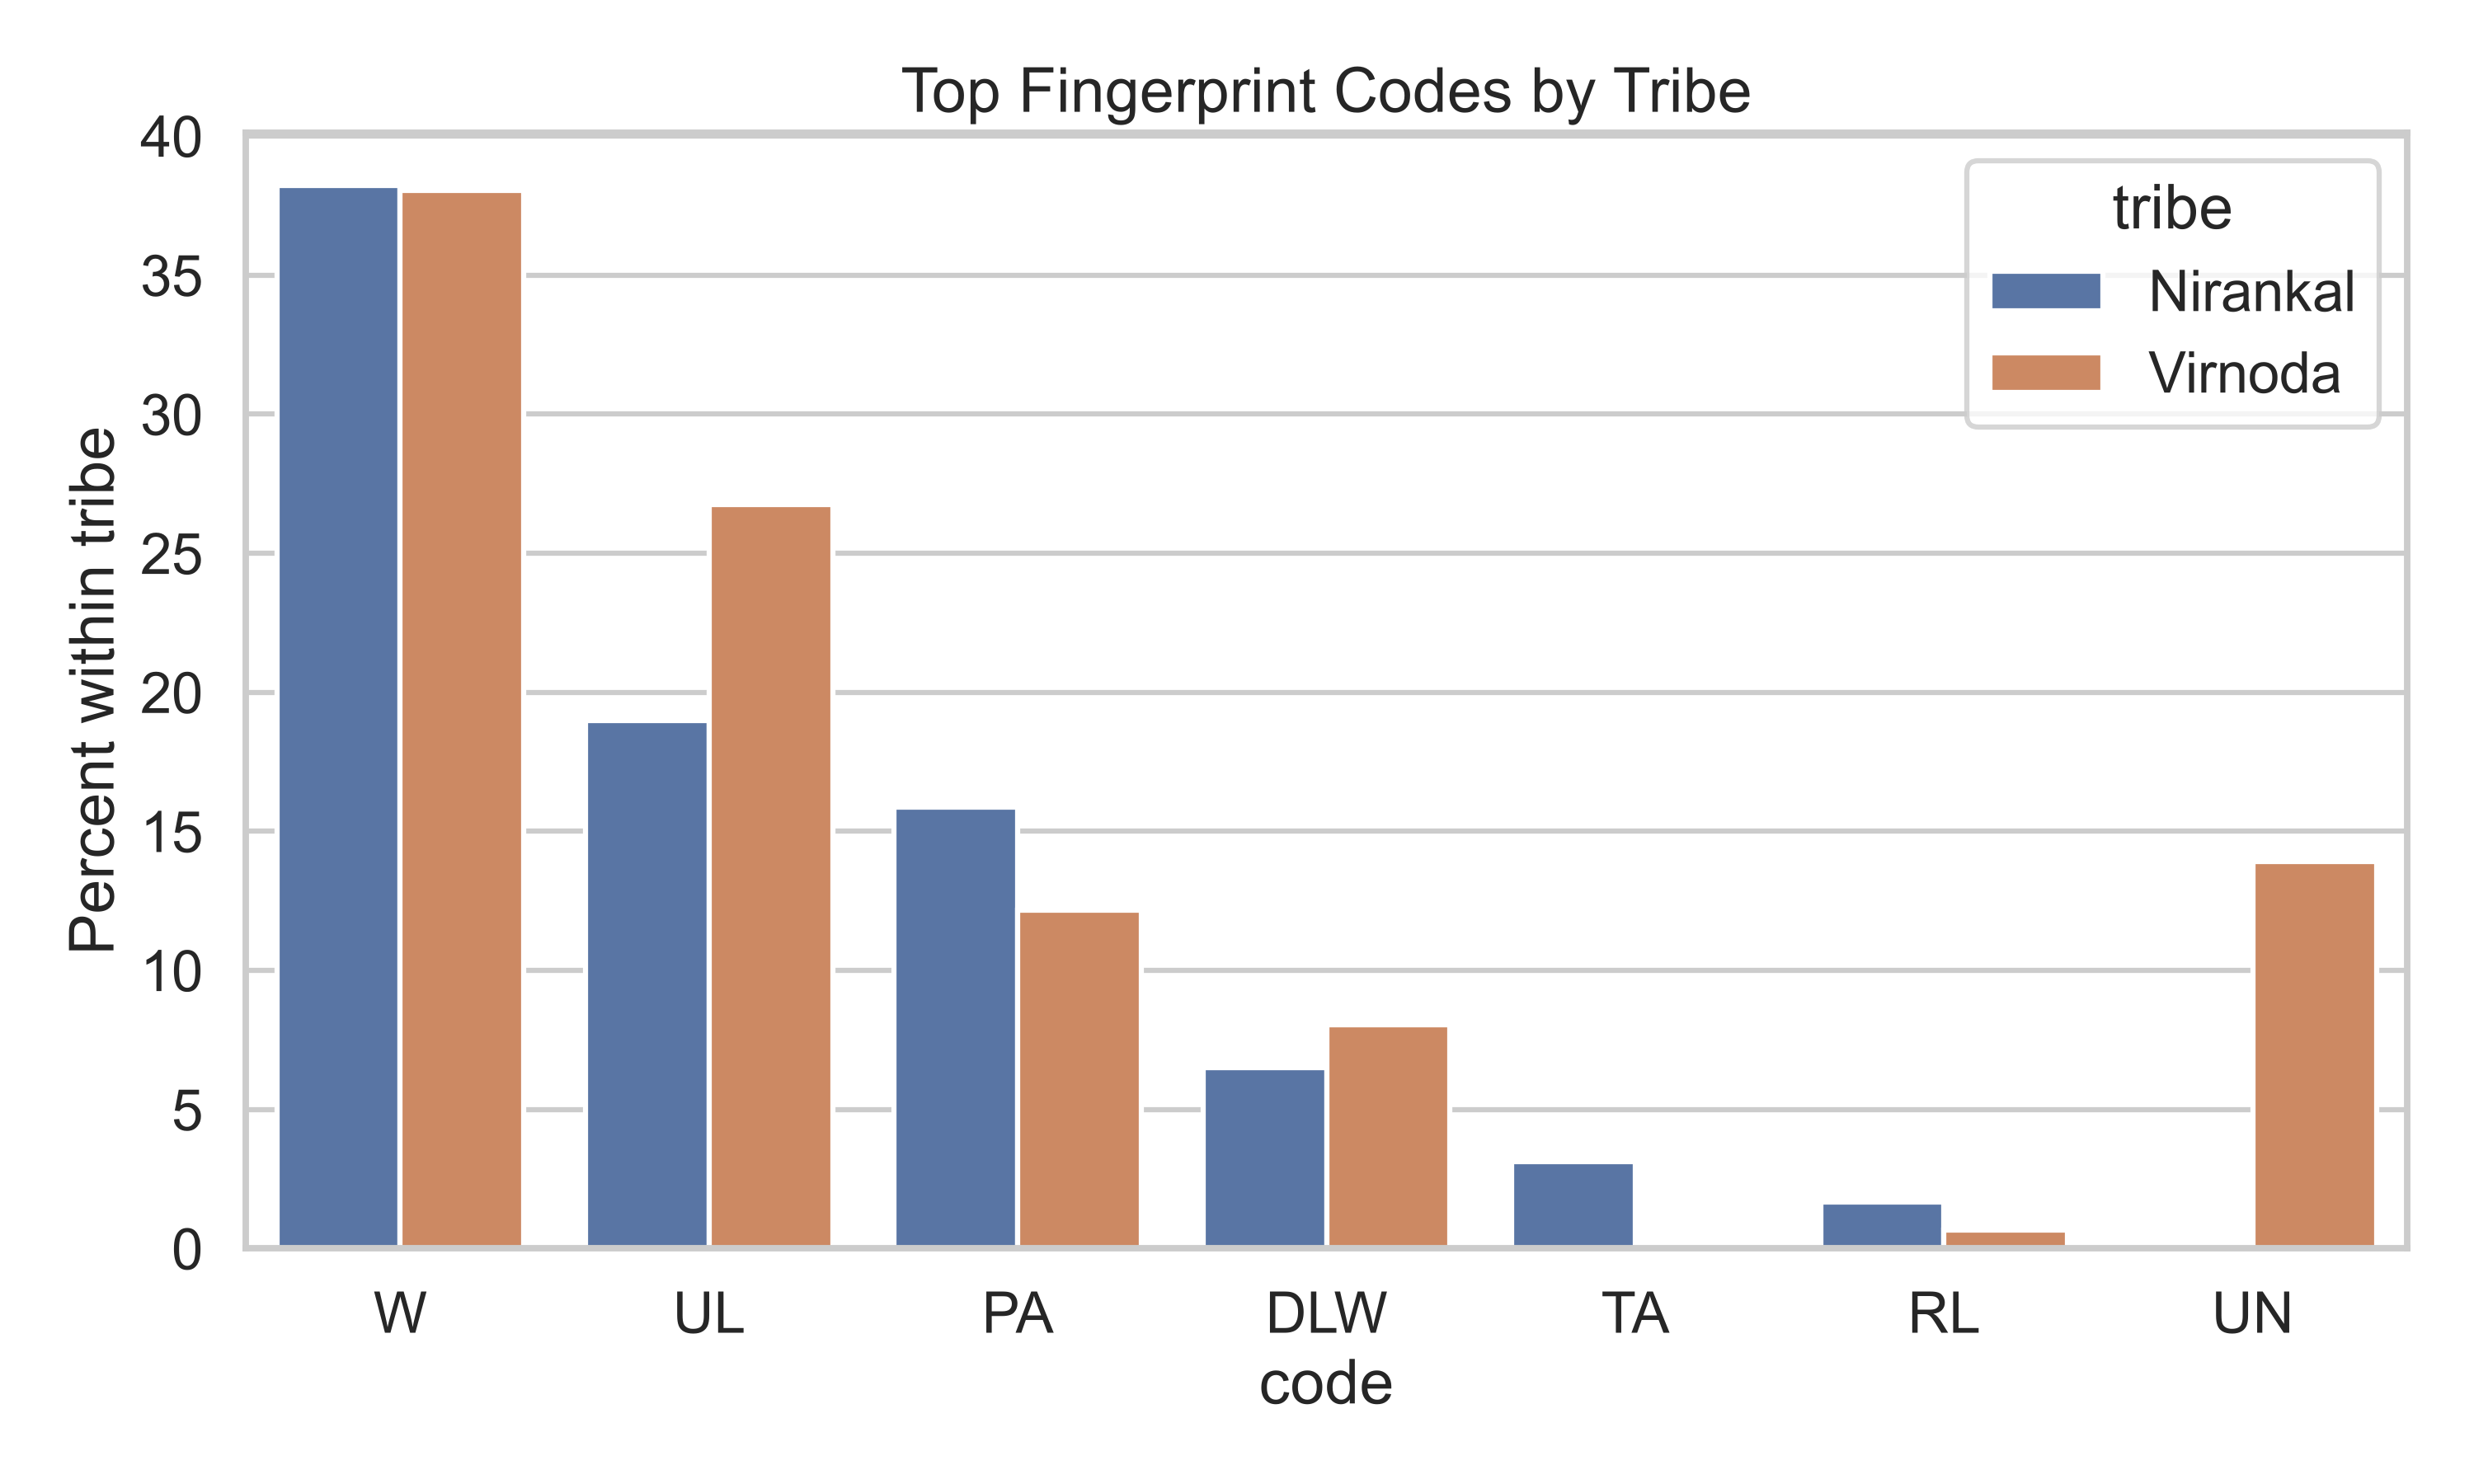
\includegraphics[width=0.85\textwidth]{figures/fingerprint_top_codes.png}
\caption{Top fingerprint code composition by tribe.}
\label{fig:fptop}
\end{figure}

\begin{figure}[H]
\centering
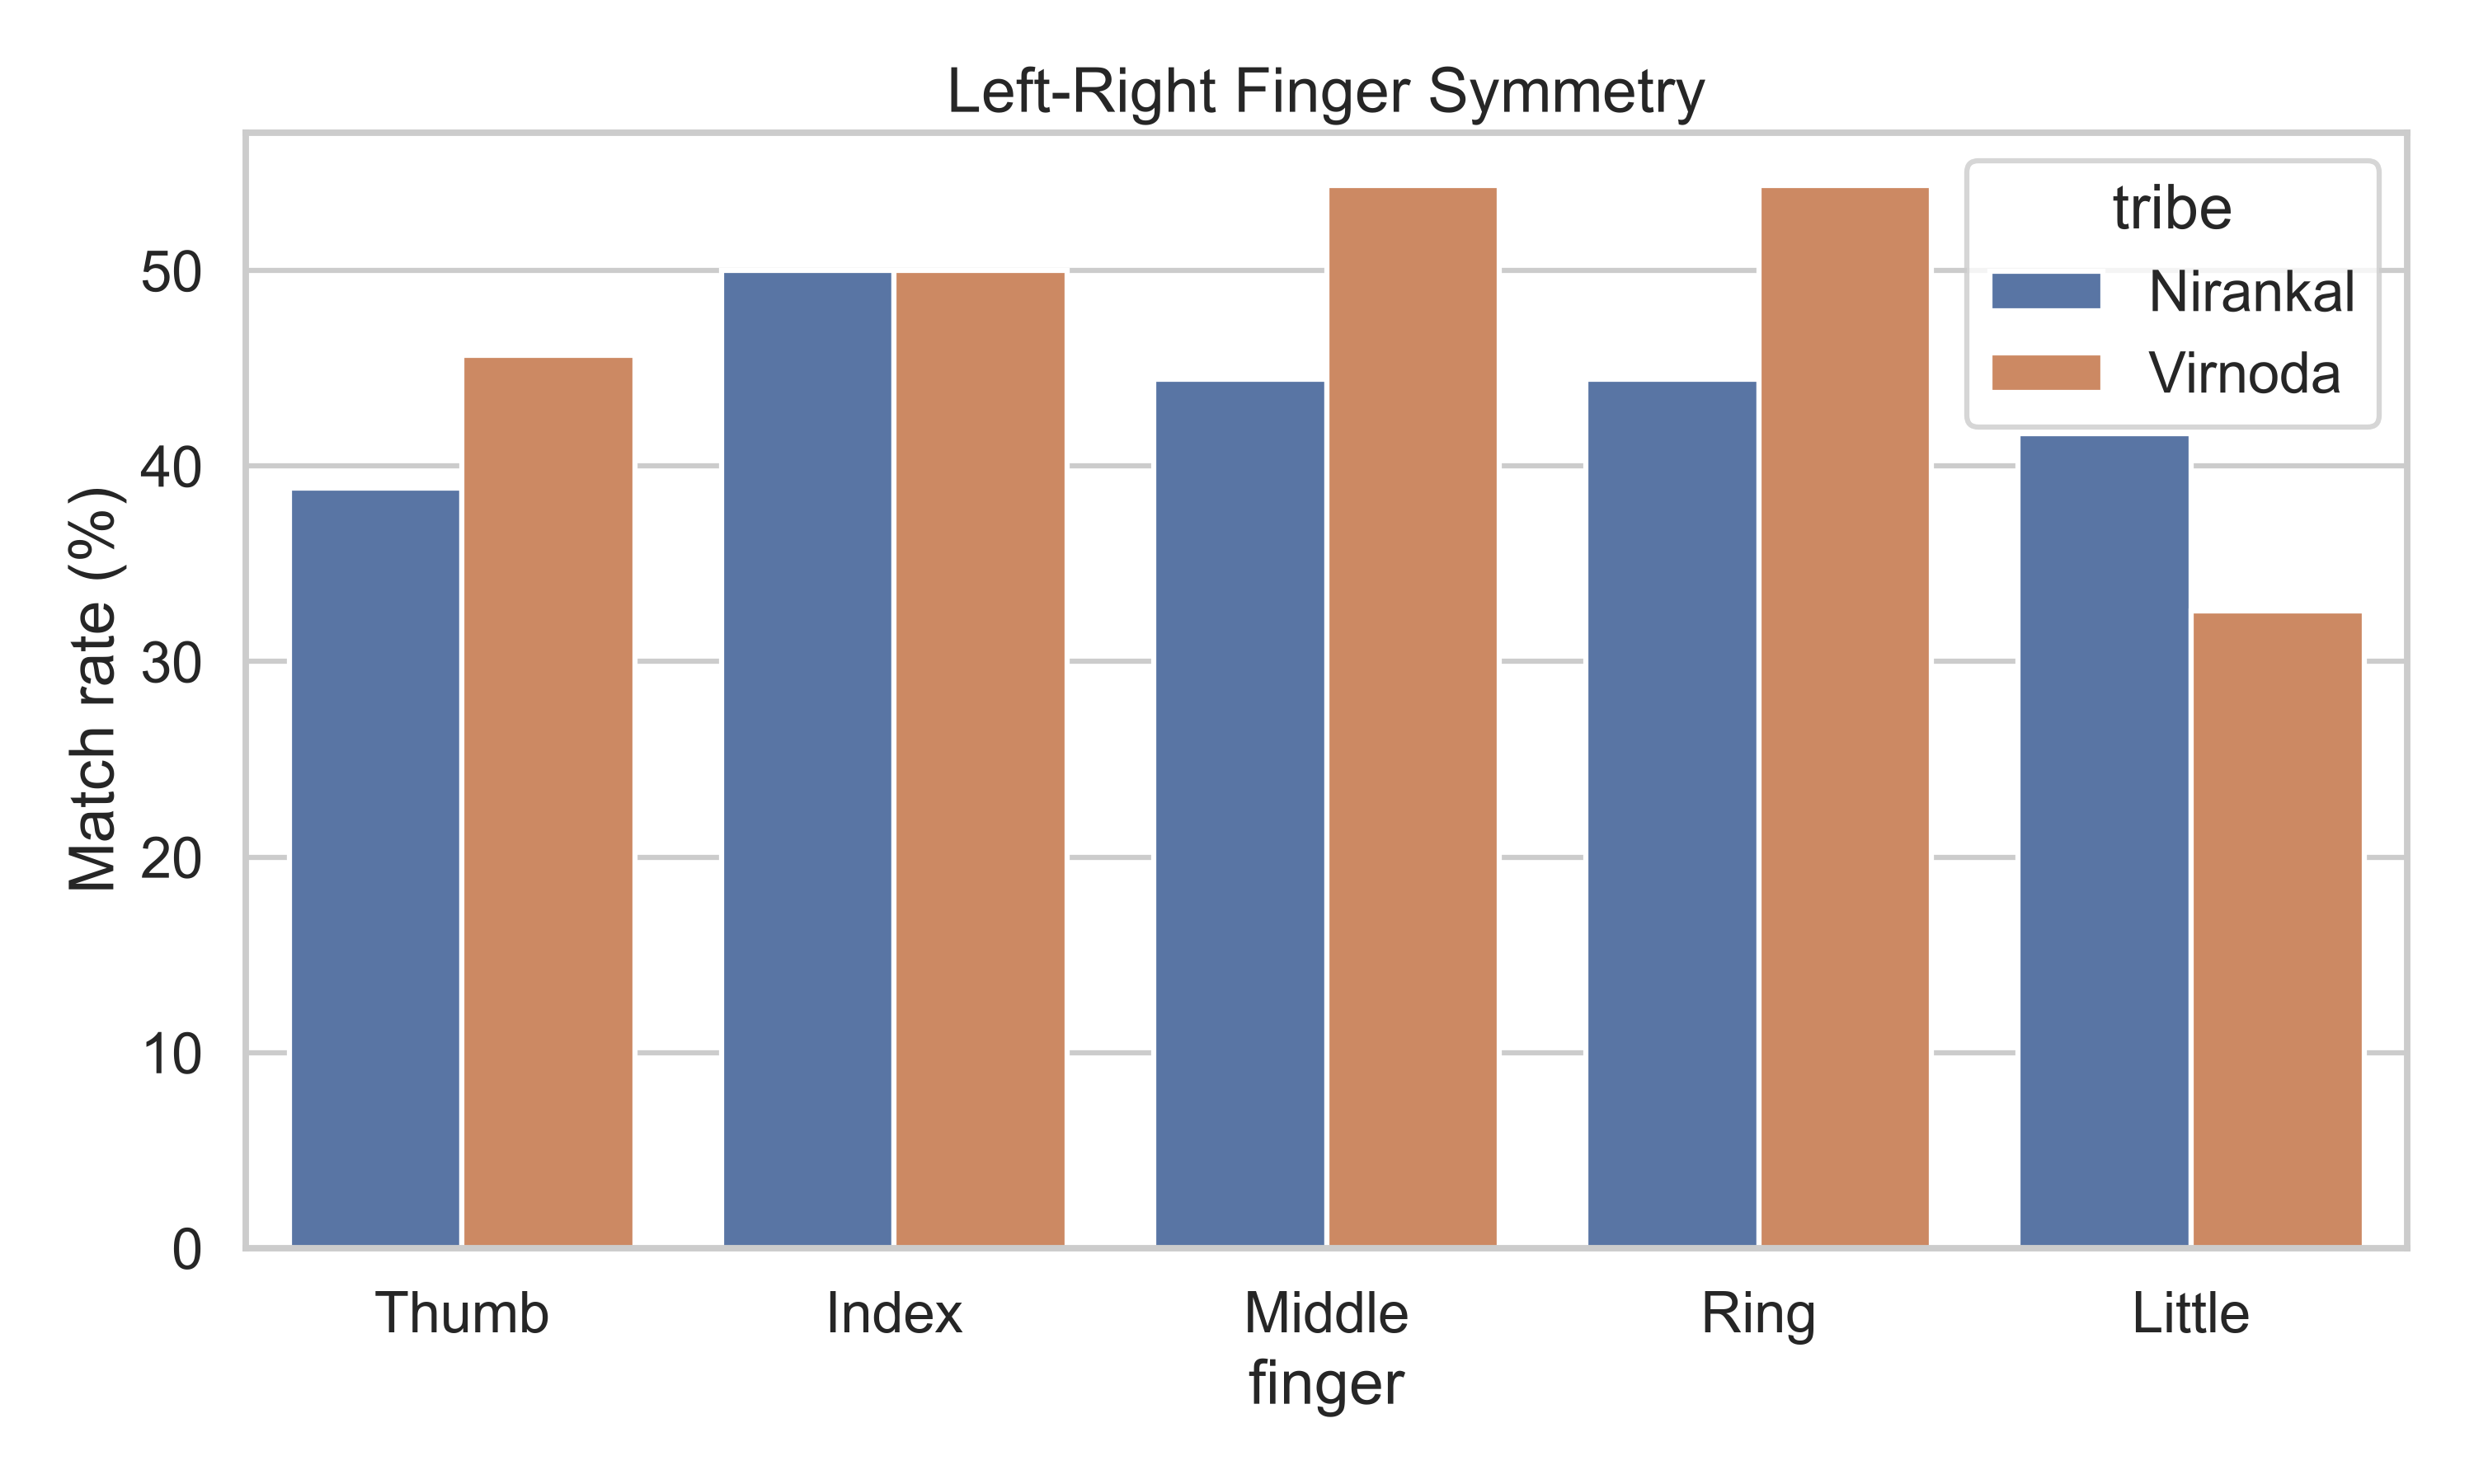
\includegraphics[width=0.85\textwidth]{figures/fingerprint_symmetry.png}
\caption{Left-right same-finger symmetry rates by tribe.}
\label{fig:symm}
\end{figure}

\subsection{Multivariate geometric structure}
PCA of anthropometric variables yielded partially overlapping tribe clouds with directionally shifted centroids rather than fully separated clusters (Figure~\ref{fig:pca}). This supports interpretation of the cohort contrast as a profile displacement with high shared variance, not strict partitioning.

\begin{figure}[H]
\centering
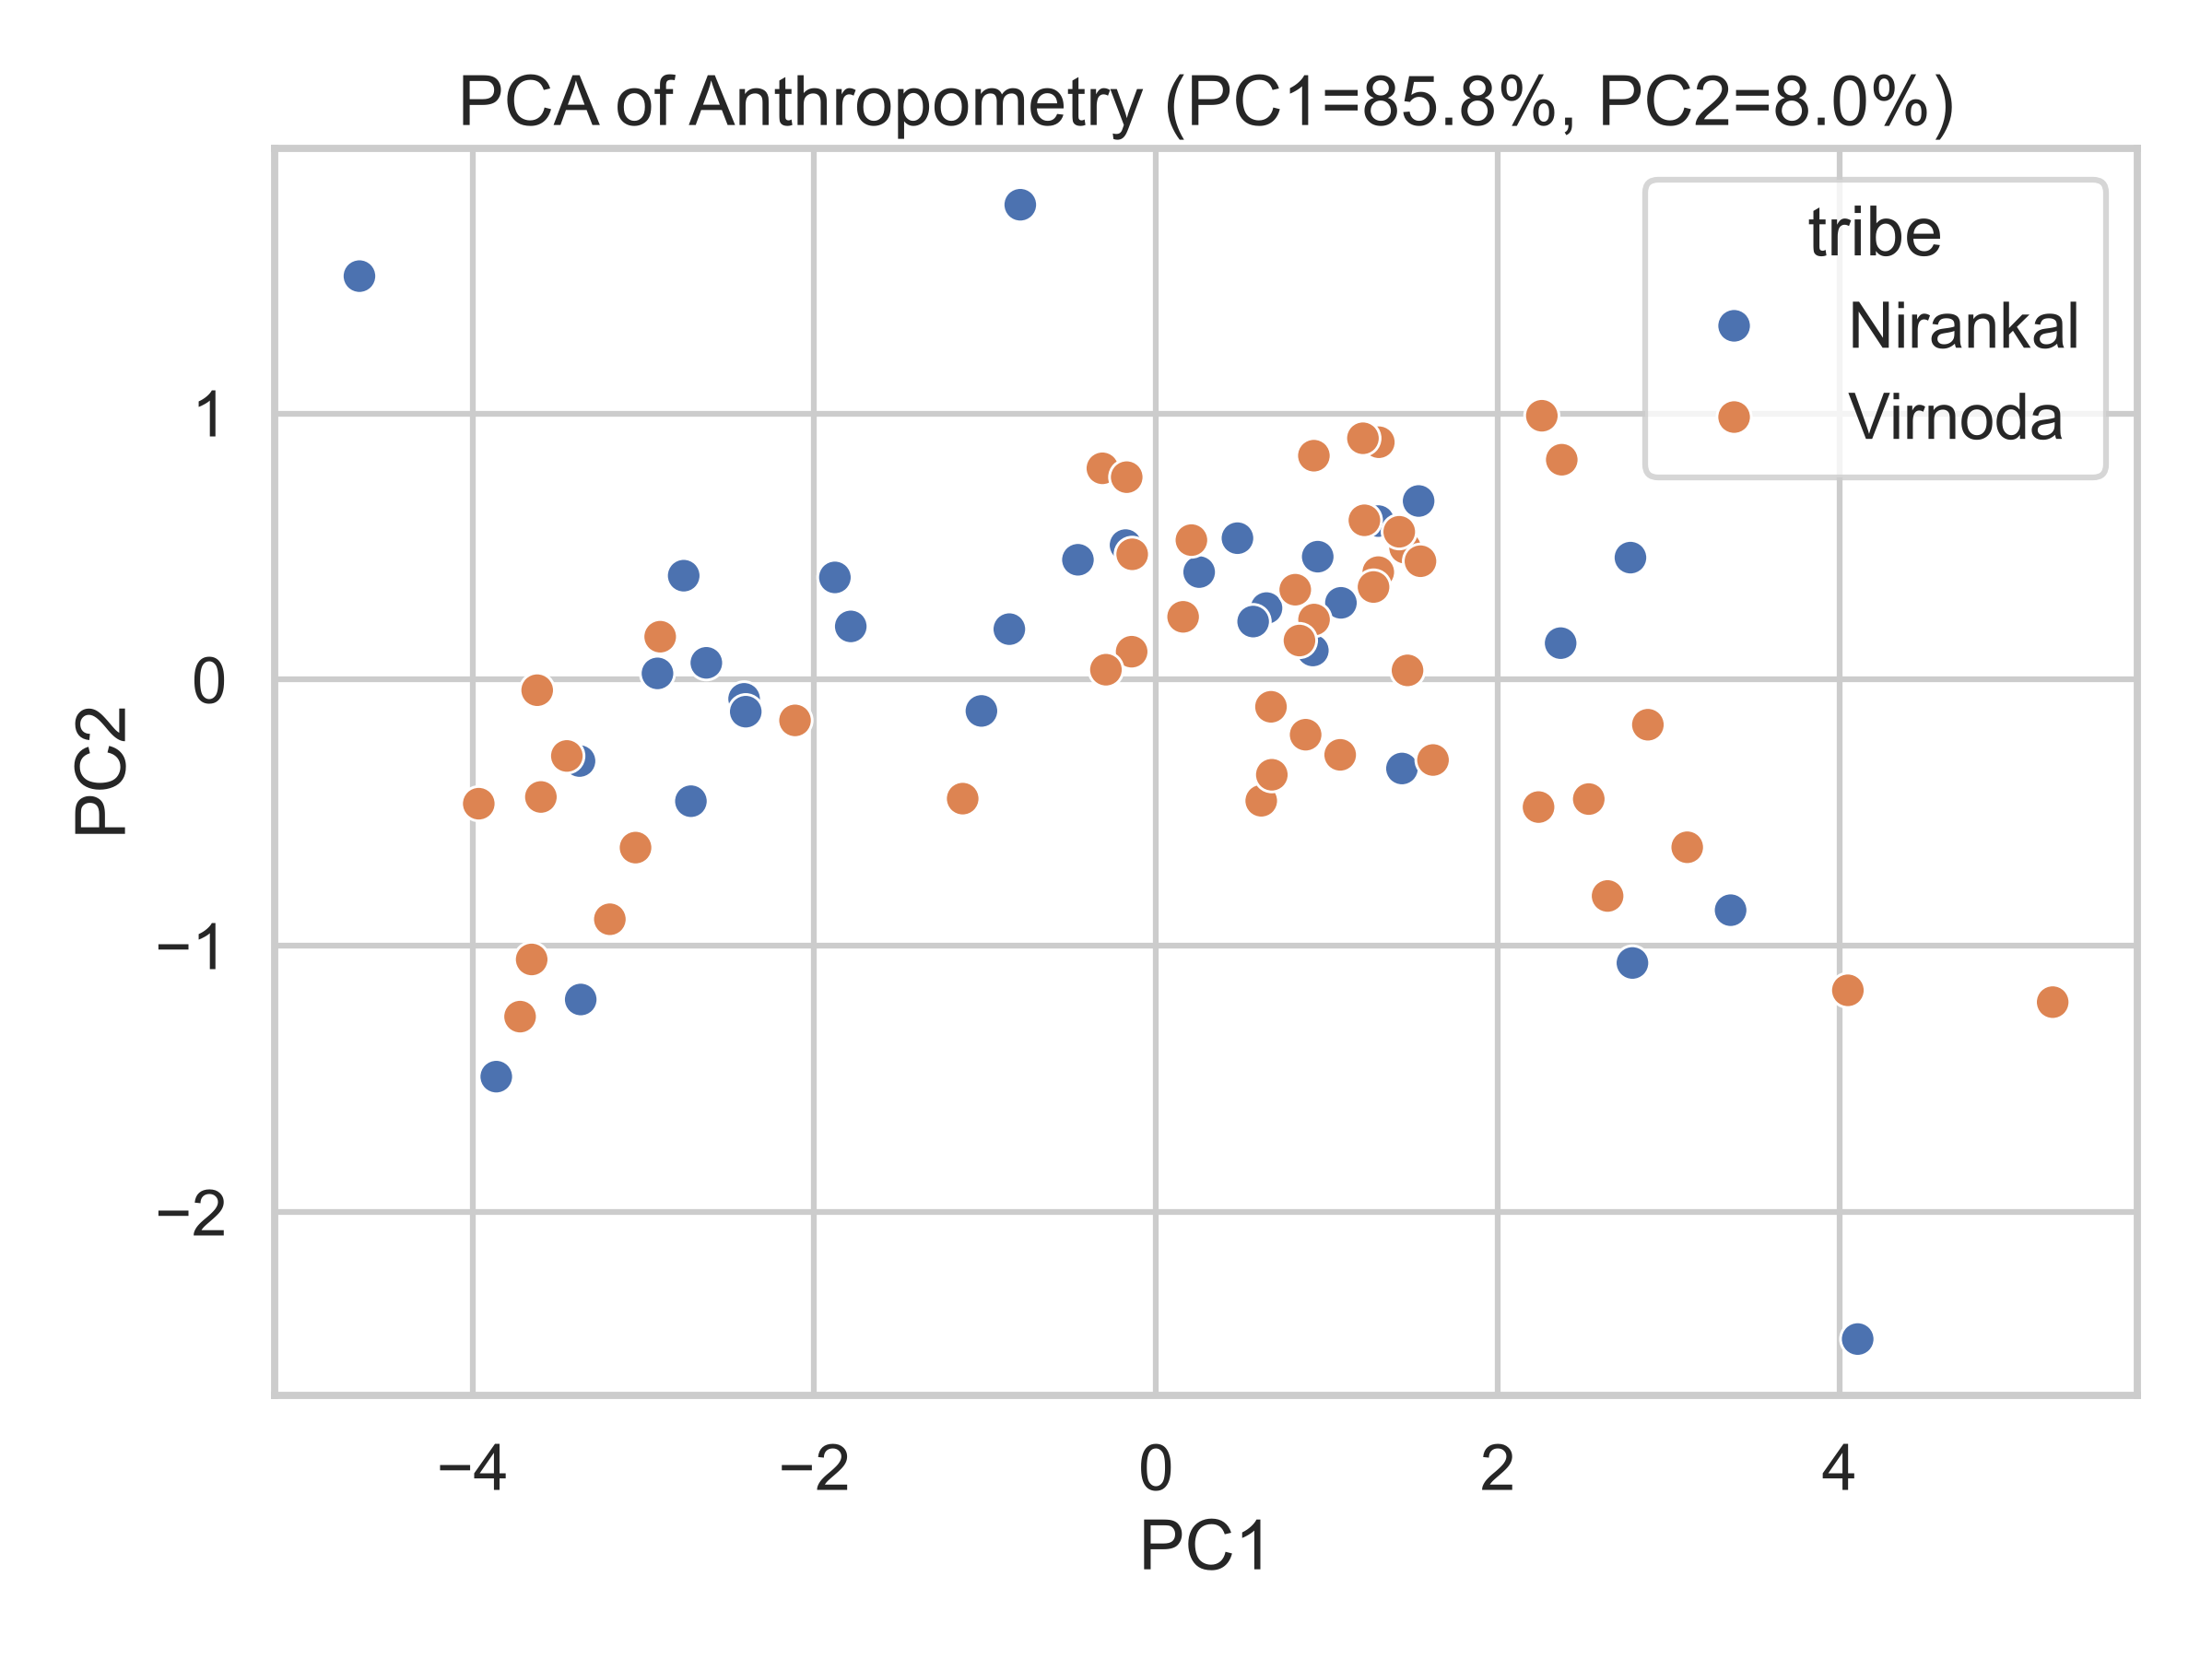
\includegraphics[width=0.75\textwidth]{figures/anthropometry_pca.png}
\caption{PCA projection of anthropometric features.}
\label{fig:pca}
\end{figure}

\subsection{Data quality context}
Missingness varied by domain and tribe (Table~\ref{tab:missing}), with the highest incompleteness in fingerprint-hair and questionnaire layers. This reinforces the need to interpret behavioral and microstructure inferences with domain-specific caution.

\begin{table}[H]
\centering
\caption{Dataset-level missingness profile.}
\label{tab:missing}
\begin{tabular}{llrrr}
\toprule
Tribe & Dataset & Rows & Columns & Missingness (\%) \\
\midrule
Nirankal & roster & 120 & 3 & 0.56 \\
Virnoda & roster & 68 & 3 & 0.98 \\
Nirankal & measurements & 53 & 30 & 10.75 \\
Virnoda & measurements & 68 & 30 & 13.82 \\
Nirankal & questionnaire & 36 & 26 & 51.18 \\
Virnoda & questionnaire & 51 & 26 & 53.32 \\
Nirankal & fingerprint\_hair & 83 & 32 & 58.77 \\
Virnoda & fingerprint\_hair & 104 & 32 & 50.84 \\
\bottomrule
\end{tabular}
\end{table}

\section{Discussion}
Three principal conclusions emerge. First, cross-tribe differences are detectable but generally moderate in anthropometric magnitude, with effect-size signatures suggesting practical overlap despite directional shifts. This pattern is consistent with many community observational contexts where environmental and developmental gradients alter central tendencies while preserving substantial within-group variance.

Second, behavioral variables, especially tobacco-use response patterns, carry stronger discriminative signal than many body metrics in this dataset. Given missingness and potential reporting bias, these findings should be interpreted as a population-level indicator pattern rather than a direct prevalence estimate.

Third, dermatoglyphic composition shows meaningful diversity asymmetry despite shared dominant classes. The entropy contrast and finger-level symmetry differences support the value of retaining dermatoglyphic features in integrated community profiling frameworks.

Methodologically, our results highlight why a single-test strategy is insufficient for survey-derived tribal datasets. Combining robust non-parametric tests, categorical association, effect-size reporting, multiplicity adjustment, and multivariate projection produces a more faithful representation of both similarity and divergence.

\section{Limitations}
This work uses secondary spreadsheet records with varying completion rates across domains. Some categories are sparse, which inflates uncertainty in contingency analyses. Fingerprint coding appears to include mixed symbolic and numeric entries in places, requiring normalization and careful interpretation. External covariates (socioeconomic status, geography, migration history, dietary biomarkers) were not available for adjustment.

\section{Conclusion}
An integrated analysis of Nirankal and Virnoda data indicates that cross-tribe structure is multidimensional: demographic and anthropometric shifts are present but modest, behavioral responses provide stronger divergence in specific domains, and dermatoglyphic diversity patterns differ despite common dominant classes. The presented pipeline offers a reproducible, publication-oriented template for future tribal health and biosocial studies.

\section{Data availability}
All analyzed source workbooks were provided within the project workspace. Derived analysis tables and manuscript figures are available under \texttt{paper\_assets/tables} and \texttt{paper\_assets/figures}.

\section{Code availability}
All scripts used for harmonization, inference, and figure generation are included in the project workspace, including \texttt{generate\_paper\_assets.py} and the Streamlit analytical interface.

\section{Author contributions}
Ranji Kolkar conceived the study, curated data structures, and supervised analysis. Swea Nidhi designed and executed the statistical pipeline, generated figures and tables, and drafted the manuscript. Both authors interpreted results, revised the article, and approved the final version.

\section{Competing interests}
The authors declare no competing interests.

\bibliography{references}

\end{document}
